% This is LLNCS.DEM the demonstration file of
% the LaTeX macro package from Springer-Verlag
% for Lecture Notes in Computer Science,
% version 2.4 for LaTeX2e as of 16. April 2010
% 
\documentclass{llncs}
%
\usepackage{makeidx}  % allows for indexgeneration
\usepackage{amsmath}
\usepackage{amssymb}
\usepackage{graphicx}
\usepackage{tikz}

%
\begin{document}
%
\mainmatter              % start of the contributions
%
\title{An Executable Formal Semantics For A Functional Actor Language}
%
\author{Xiaohong Chen, Lucas Pe\~{n}a}
%
\institute{University of Illinois at Urbana-Champaign, \\
\email{\{xc3,lpena7\}@illinios.edu}}

\maketitle              % typeset the title of the contribution

\begin{abstract}
A simple reference actor language has been proposed in~\cite{actor}, serving as a
sound mathematical calculus foundation for various actor languages used in
distributed applications that involves concurrency. Even though the authors
of~\cite{actor} provided in the paper an operational semantics of the actor language,
an executable implementation was not given. In this project, we will give the
reference actor language an implementation that by construction conforms to its
formal operational semantics using the K framework~\cite{kframework}, a rule-based
semantic framework. We will show that our executable formal semantics are
capable of executing some meaningful actor systems examples. We hope our
executable formal semantics can be served as a starting point for future work in
developing automatic equivalence provers using the K framework.
\end{abstract}
%
\section{Introduction}
The K framework~\cite{kframework} is a framework for defining executable operational
semantics of a programming language. K is based on rewriting logic, organizing
the state of a program into cells and rewriting the particular parts of the
configuration. K also has access the entire computation at any particular
time. These features and more allow for difficult language constructs to be
designed with ease in K. On top of that, K provides backend tooling for
additional features based on the semantics of a programming language, such as a
semantic debugger and a full formal verifier. See Figure~\ref{fig:k-tools} for a
complete view of the tools one gets from K based off an operational semantics.

In the rest of the paper we discuss related work, then the actor semantics in
some detail, including the configuration, the syntax and how we handle reduction
contexts in K, the semantics, and an in-depth example. We then conclude and
discuss future work.

\section{Related Work}

\begin{figure}
  \centering
  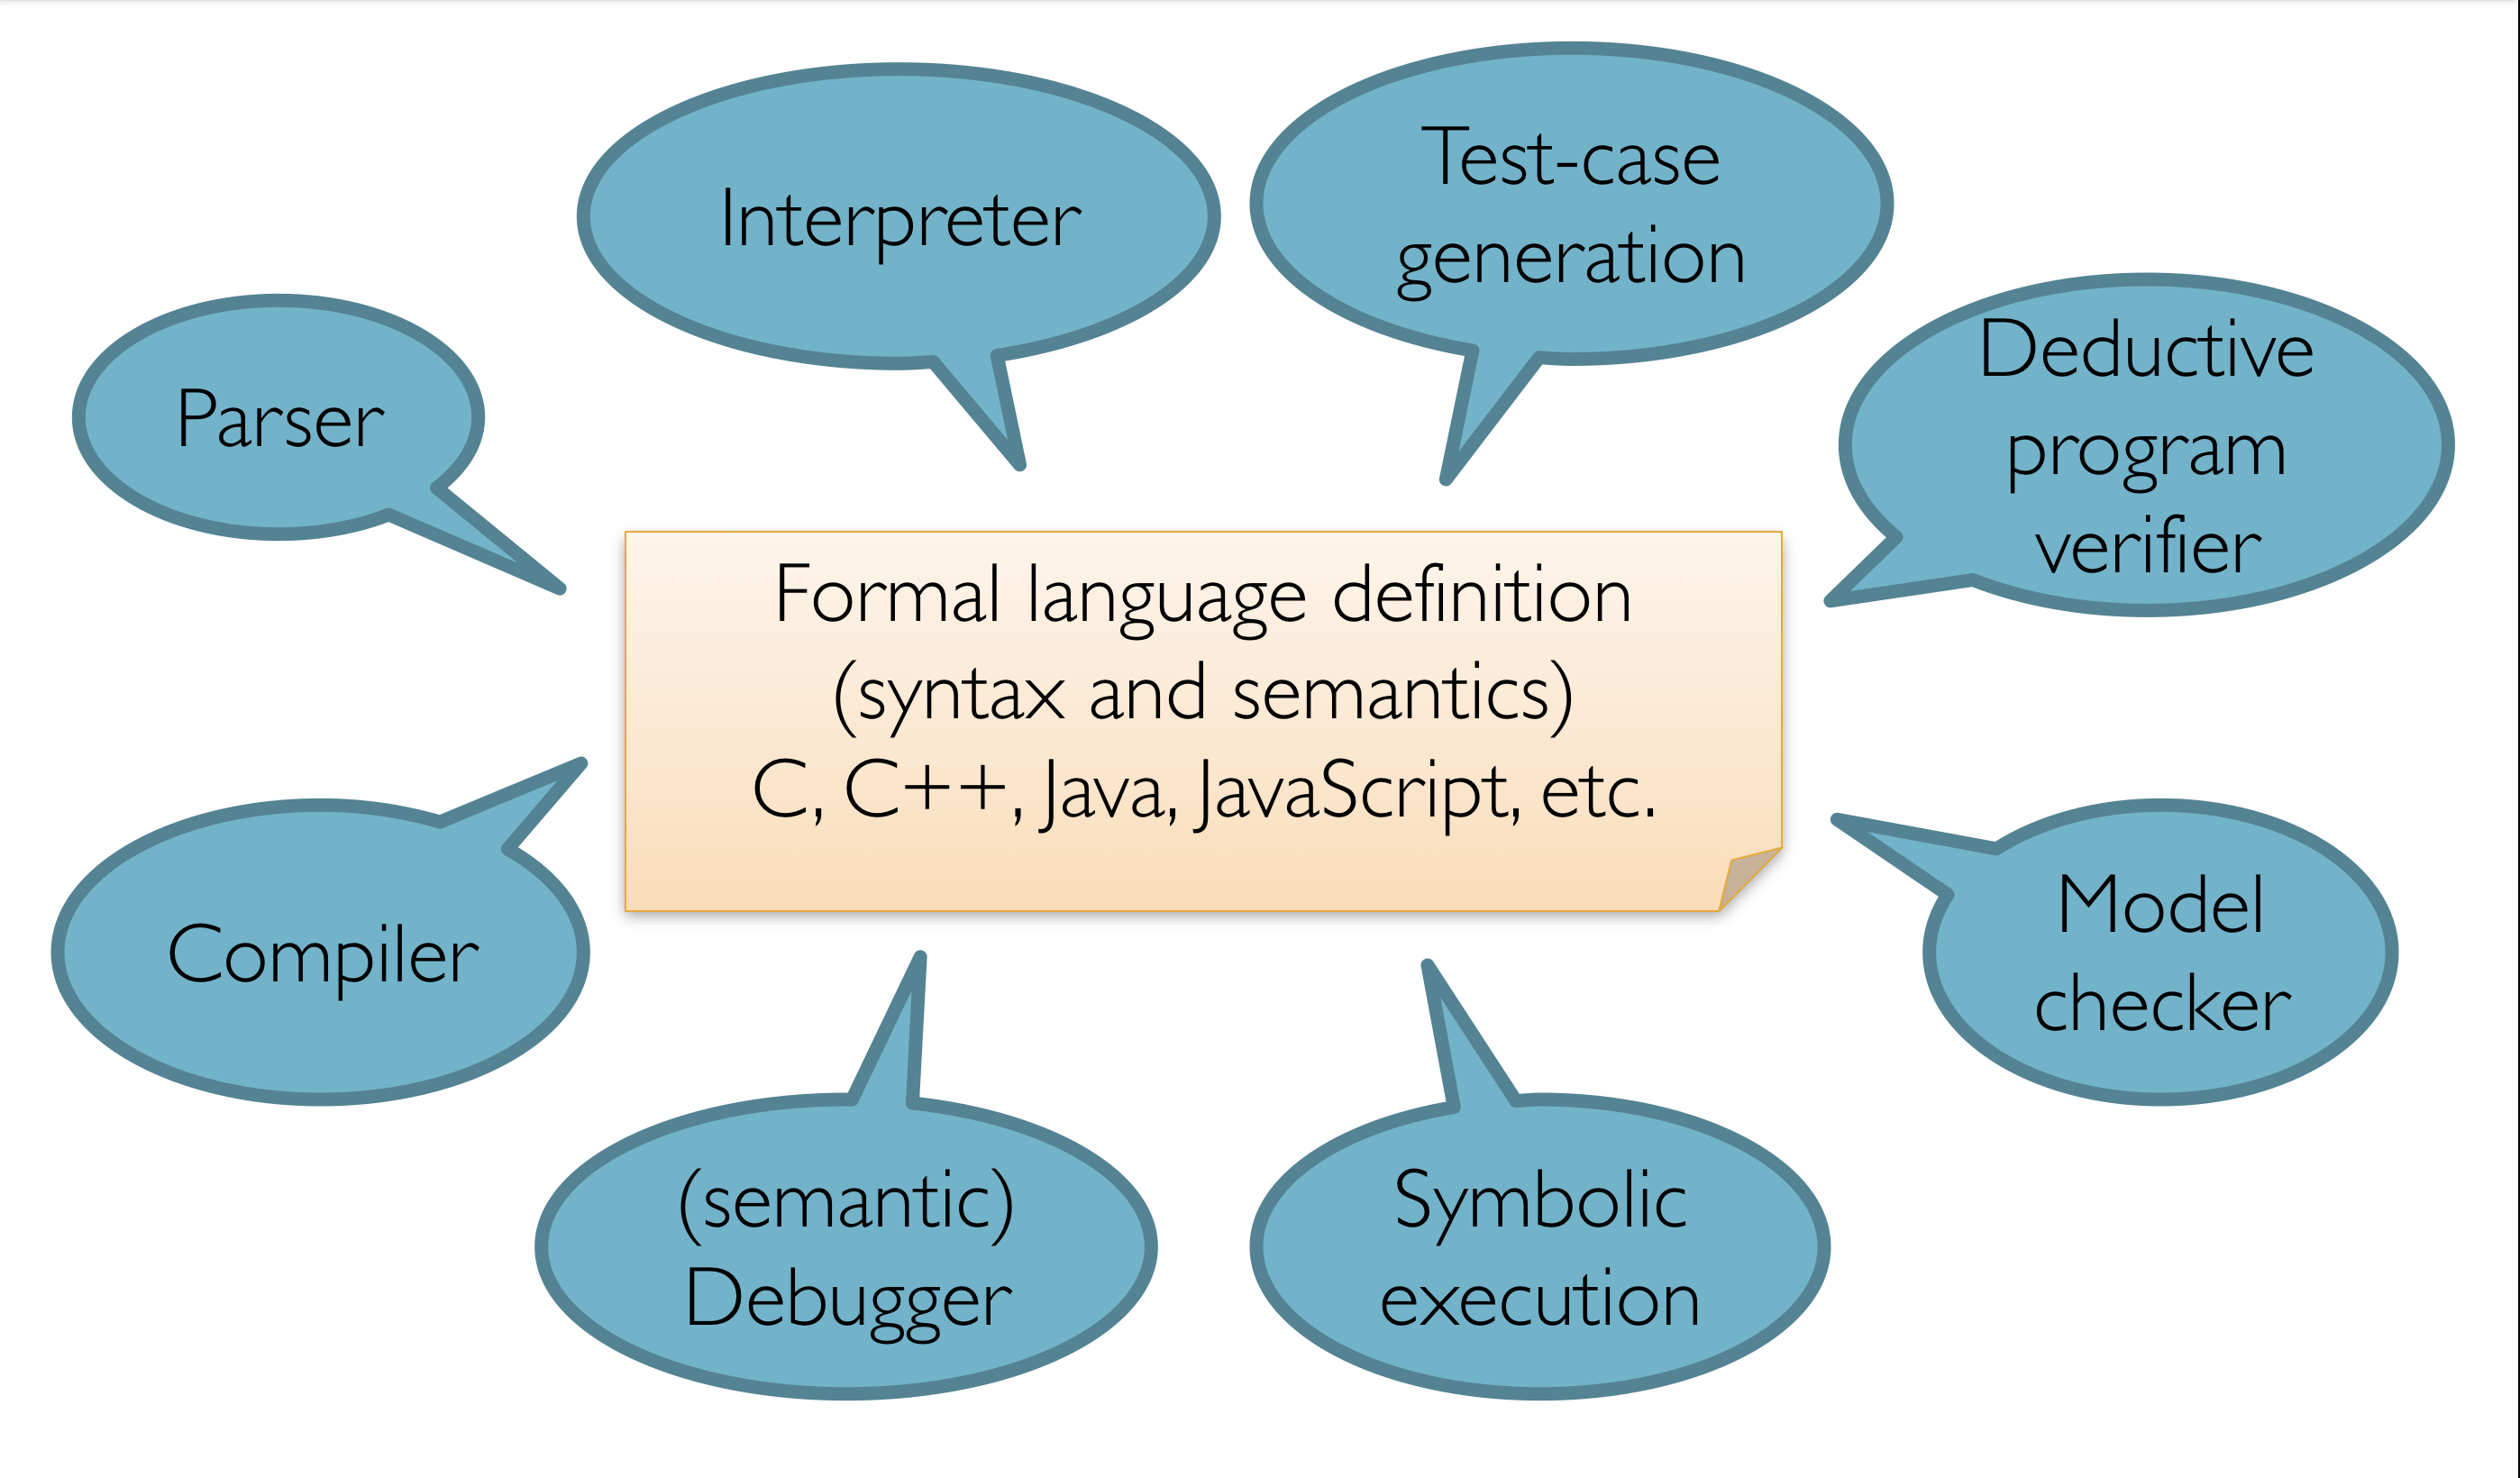
\includegraphics[width=0.8\textwidth]{../k-overview.png}
  \caption{Backend tools K provides from just an operational
           semantics. Some tools such as a semantics-based compiler and
           test-case generation are in progress.}
  \label{fig:k-tools}
\end{figure}
To demonstrate the power of K, languages as complex as C, Java, and JavaScript
have been fully defined using the K framework~\cite{kc,kjava,kjs}. On top of that, in
all of these languages and more, nontrivial programs have been formally verified
using K's prover, such as proofs involving AVL trees and red-black trees. We
would like to add an actor-based language to the growing list of languages
defined in K, so we can take advantage of K's formal verification engine and
more.

Semantics of actor-based languages have been defined on paper, for example
in~\cite{actor}. Additionally, there are many implementations of actor-based systems,
including Erlang~\cite{erlang}, Akka~\cite{akka}, Scheme~\cite{scheme}, and much more. However,
there is currently no formally defined \emph{executable} operational semantics
of an actor-based language. In K, there was previous work done to define the
semantics of Orc, a concurrent programming language~\cite{orc}, though that work is
incomplete.

In this paper, we aim to define the semantics of the actor language proposed
in~\cite{actor}.  We choose this language as the semantics are clearly defined in the
paper, and it is one of the more simple actor frameworks. Defining this language
in K will give assurance to the correctness of the language - as K is executable
this can be tested much easier than defining a language on paper. It will also
provide more assurance on K's language-defining ability, as well as open up to
formal analysis using the tools seen in Figure~\ref{fig:k-tools}.

\section{The Actor Language in K}
In this section, we describe in detail some important features of the actor
language from~\cite{actor}. We cover some important features from K and how 
they were
used to define key concepts of the actor language.

\subsection{Configuration}\label{sec:configuration}
All languages in K use a configuration to specify the current state of a
program. For simple languages like the lambda calculus or a simple \texttt{IMP}
language, there may only be one cell to hold the current computation (the
\texttt{<k>}\ \dots\ \texttt{</k>} cell) which is required for all languages
defined in K. For the actor language, we have the following configuration:
\begin{verbatim}
  configuration 
    <T>
      <actors>
        <actor multiplicity="*">     // a multiset of actors
          <k> exec($PGM:Exp) </k>    // actor state
          <id> initactor </id>       // actor id
        </actor>
      </actors>
      <messages>
        <message  multiplicity="*">  // a multiset of messages
          .K
        </message>
      </messages>
      <definedaddr>                  // list of defined actors'
        ListItem(initactor)          // addresses
      </definedaddr>
    </T>
\end{verbatim}
In addition to defining the state of a program, the configuration is also used
to define the initial state of a program. Initially, we only have one actor,
with the unique identifier \texttt{initactor}. It also contains the program in
the \texttt{exec} state ready to be executed. The variable \texttt{\$PGM} comes
from an external file. The notation \texttt{multiplicity=*} is used to specify
that there can be any number of \texttt{actor} cells and \texttt{message} cells
as a multiset of actors and messages respectively. Initially there are no
messages, represented using K's builtin \texttt{.K}. Finally, the
\texttt{definedaddr} cell is used to keep track of addresses of defined
actors. We need to keep track of this for the side condition of some semantic
rules (see Section~\ref{sec:semantics}).

For our K definition, we only define a single actor system, so there are no
external actors or receptionists. To add these one can simply add these as
additional cells in the configuration, initialized to the empty list.

\subsection{Syntax and Reduction Contexts}
Syntax for constructs in K is specified using BNF notation. For example, we
specify values (where reduction can no longer happen) as
\begin{verbatim}
  syntax Val  ::= CVal                                    
                | "lambda" "(" Id "," Exp ")" [binder]
                | "pr" "(" Val "," Val ")"
\end{verbatim}
where \texttt{CVal} represents the communicable values, \texttt{lambda}
represents lambda expressions, and \texttt{pr} represents pairs of values.  The
\texttt{binder} attribute is used in K's backend for substitution, as it
specifies that \texttt{Id} is bound in the term \texttt{Exp}.

In K, we can also use syntax to express contexts in which reduction is allowed.
In the actor language, reduction contexts are separately defined to specify
evaluation order of expressions. For example, the set of reduction contexts for
functions in the actor language are specified as
\[ \mathbb{F}_{n+m+1}(\mathbb{V}^n,\mathbb{R},\mathbb{E}^m) \]
This states that the argument of a function can be evaluated only when the first
$n$ arguments have already been evaluated. In K, this is simply specified using
the attribute \texttt{seqstrict} which states the arguments of a syntactic
construct are evaluated in order. Addition, for example, is specified in K as
\begin{verbatim}
  syntax Exp ::= "add" "(" Exp "," Exp ")" [seqstrict]
\end{verbatim}
Note nothing beyond the appropriate strictness attribute is needed to specify
reduction contexts in K for this language.

For the branching, we would like to only specify that only the first argument
should reduce to a value, to avoid reduction in the branch we end up not taking.
In the actor semantics from~\cite{actor}, this is accomplished with the following:
\[ \texttt{if}(e_0, e_1, e_2) \;\;\;\text{abbreviates}\;\;\; \texttt{app}(\texttt{br}(e_0, \lambda z.e_1, \lambda z.e_2), \texttt{nil}) \;\;\;\text{for $z$ fresh} \]
Notice that the second and third arguments in the branch construct are lambda
expressions, which are values, and thus will not be reduced any farther. In our
K semantics, we emulate this, but we could also define \texttt{br} directly to
be only strict in the first argument as follows:
\begin{verbatim}
  syntax Exp ::= "br" "(" Exp "," Exp "," Exp ")" [strict(1)]
\end{verbatim}
Strictness constructs like this avoid unnecessary syntactic sugar, and cleanly
specify most reduction contexts one would require.

\subsection{Semantics}\label{sec:semantics}
Semantics in K is given as \emph{rewriting rules} of the form $l \Rightarrow r$.
For example, the  beta-reduction rule (beta-v) is specified as
\begin{verbatim}
  rule app(lambda(X:Id, E:Exp), V:Val) => E [ V / X ]
\end{verbatim}
where \texttt{E [ V / X ]} is the result of substituting \texttt{V} for 
\texttt{X} in \texttt{E} using K's internal substitution mechanism.
K rules start with the keyword \texttt{rule}. The left hand side of the rule 
and right hand side of the rule are separated by a double arrow~``\texttt{=>}''.

Conditional reduction rules can also be easily specified.
For example, the branching rule (br) is specified as two K rules
\begin{verbatim}
  rule br(nil, V1:Val, V2:Val) => V2
  rule <k> br(V:Val, V1:Val, V2:Val) => V1 ... </k>
       <definedaddr> X </definedaddr>
    requires notBool((isId(V) andBool notBool(V in X))
                              orBool V ==K nil)
\end{verbatim}
The first rule says if the first argument is \texttt{nil}, the branching 
operator \texttt{br} returns its third argument.
The second rule is a bit complicated.
It says if the first argument is neither \texttt{nil} nor an
unknown address, the branching operator \texttt{br} returns its second
argument.
The \texttt{requires} keyword is used to specify rewriting conditions that 
decide when a rewrite rule can be applied.

The single-step transition relation $\mapsto$ on actor configurations is 
similarly specified using K rules.
For example, the \texttt{<init: a, a1>} transition rule is specified as
\small
\begin{verbatim}
  rule <actor>
         <k> initbeh(A1, V:Val) => nil ... </k>
         <id> A </id>
       </actor>
       <actor>
         <k> uninit(A) => ready(V) ... </k>
         <id> A1 </id>
       </actor>
\end{verbatim}
\normalsize
The rule involves two actors as there are two actor cells 
\texttt{<actor>}\ \dots\ \texttt{</actor>} in the rule.
The first actor is the \emph{initializer} actor while the second is the actor 
\emph{being initialized}.
K supports to only specify components that are relevant to the rule. This is 
known as the \emph{framing principle}.
The initializer actor executes \texttt{initbeh(A1, V:Val)} and gets value 
\texttt{nil}, as specified in the rule.
The rest of the computation or so-called \emph{reduction context} is unchanged and
kept in 
the following~``\texttt{...}''.

Reduction contexts can be mentioned explicitly when needed.
For example, in the following \texttt{<bec: a, a1>} rule,
\small
\begin{verbatim}
  rule <actor>
         <k> (become(V:Val) ~> RestComputation) => ready(V) </k>
         ...
       </actor>
       (.Bag => <actor>
                  <k> nil ~> RestComputation </k>
                  <id> !A1:Id </id>
                </actor>)
       <definedaddr> Ads => Ads ListItem(!A1) </definedaddr>
\end{verbatim}
\normalsize
the reduction context \texttt{RestComputation} is explicitly passed to a 
newly-generated actor with a fresh identity \verb|!A1|.
The tilde arrow expression \verb|T ~> R| 
means the decomposition \verb|R[T]| with reduction context \texttt{R} and redex 
\texttt{T}.

\subsection{In-depth Example}
We test our actor semantics on many examples. One of the more complicated test
cases is an example of tree recursion~\cite{actor}.  The problem is to calculate
the product of all leaves of a binary tree.  The problem is solved by a
divide-and-conquer algorithm which calculates the results for two subtrees and
multiplies the results.  The algorithm is implemented using a
\emph{join continuation} as follows.
\small
\begin{verbatim}
let(bind(sink,
  rec(lambda(b, lambda(m, become(b))))),
let(bind(ident,
  lambda(m, m)),
let(bind(joincont,
  rec(lambda(b, lambda(c, lambda(nargs, lambda(firstnum, lambda(num,
    if(eq?(nargs, 0),
       become(app(app(app(b, c), 1), num)),
       seq(become(sink),
           send(c, mult(firstnum, num))))))))))),
let(bind(treeprod,
  rec(lambda(b, lambda(self, lambda(m,
    seq(become(app(b, self)),
        if(isnat(tree(m)),
           send(cust(m), tree(m)),
           letactor(bind(newcust, app(app(app(joincont, cust(m)), 0), nil)),
             seq(send(self, pr(left(tree(m)), newcust)),
                 send(self, pr(right(tree(m)), newcust))))))))))),
let(bind(tr, 
  pr(pr(1, pr(2, pr(3, 4))), pr(pr(5, 6), 7))),
letactor(
  bind(tpactor, app(treeprod, tpactor)),
  bind(custactor, ident),
  send(tpactor, pr(tr, custactor))))))))
\end{verbatim}
\normalsize

Recall that our semantics initializes the initial actor with the behavior of 
executing the above lambda expression.
Therefore after five nested \texttt{let}-expressions, the initial actor creates 
two 
actors. One is the \texttt{tpactor} that calculates the tree product.
The other is the \texttt{custactor} that receives the result.
The initial actor sends \texttt{tpactor} a message containing a binary tree 
whose leaves are $1, 2, \dots, 7$, and the address of the customer actor 
\texttt{custactor}.
When the actor system terminates, we get the following configuration
\small
\begin{verbatim}
  <T>
    <actors>
      <actor>
        <k> ready ( ... ) </k>
        <id> _93 </id>
      </actor>
      <actor>
        <k> ready ( ... ) </k>
        <id> _179 </id>
      </actor>
      .... ....
      <actor>
        <k> ready ( ... ) </k>
        <id> _45 </id>
      </actor>
      <actor>
        <k> exec ( nil ) </k>
        <id> initactor </id>
      </actor>
      <actor>
        <k> exec ( 5040 ) </k>
        <id> _46 </id>
      </actor>
      ......
      ......
    </actors>
    <messages> .MessageCellBag </messages>
    <definedaddr> ... </definedaddr>
  </T>
\end{verbatim}
\normalsize
In the configuration there are many idle actors generated during the 
computation. The customer actor, which in this execution has identity 
\texttt{\_46}, is holding the final product of 5040.

\section{Conclusion and Future Work}
\label{sec:conclusion}
In this paper we showed how to define the actor semantics from~\cite{actor} using the
K framework. We described in detail the syntax and semantics of the language in
K, as well as the configuration for our actor language. We also showed how we
can use K's strictness attributes to emulate the reduction contexts described
in~\cite{actor}. Finally, we discussed a complicated actor program, the tree product
example, and its encoding in K.

One immediate area for future work includes defining more actor programs and
more in-depth actor programs in K. Having a large test suite of complicated
examples can be used to ensure that the semantics in K and the semantics
from~\cite{actor} do not have any bugs. It can also be used to determine rule
coverage, affirming that all semantic rules can be applied.

Another important area for future work involves taking advantage of K's
backend tools for formal analysis, such as proving actor programs correct using
K's verification engine. For verification, K uses reachability logic~\cite{reachabilitylogic}, a
language-independent formal verification framework. Reachability logic supports
all-path reachability, so it can be used to verify programs involving concurrent
semantics. However, in order to fully take advantage of this verification, one
would need to implement partial-order reduction in K in order to reduce the
state space.

Finally, we would also like to extend our semantics to allow interaction between
actor systems by adding external actors and receptionists, as mentioned in
Section~\ref{sec:configuration}. This would allow us to define more complicated
programs, and it would also allow us to define programs like the tree product
program more compactly. Additionally, it would allow us to begin asking
questions regarding observational equivalence of actor systems, and perhaps even
take advantage of K's analysis tools to prove such equivalences.

%
% ---- Bibliography ----
%
\bibliographystyle{ieeetr}

\bibliography{references}

\end{document}
